\documentclass[11pt]{article}

\usepackage{graphicx} % Allows including images
\usepackage{booktabs} % Allows the use of \toprule, \midrule and \bottomrule in tables
\usepackage{amsmath}
\usepackage{amsfonts}
\usepackage{ifthen}
\usepackage{amssymb}
\usepackage{amsbsy}
\usepackage{bm}
\usepackage{ulem}
\usepackage{float}
\usepackage{latexsym}
\usepackage{comment}
\usepackage{graphicx}
\usepackage{amstext}
\usepackage{latexsym}
\usepackage{arydshln}
\usepackage{longtable}
\usepackage{enumerate}
\usepackage{multirow}
\usepackage{cases}
\usepackage{geometry}
\usepackage{mathtools}
\usepackage{subeqnarray}
\usepackage{textcomp}
\usepackage{hyperref}
%\usepackage{subfigure}
\usepackage{url}
\usepackage{threeparttable}
\usepackage{xr}
\usepackage{multirow}
\usepackage{wrapfig}
\usepackage{lscape}
\usepackage{rotating}
\usepackage{subcaption}
\usepackage{epstopdf}
\usepackage{verbatim}
\usepackage{xcolor}
\usepackage[sort&compress]{natbib}
\usepackage{bm}

\usepackage{algorithm}
\usepackage{algorithmic}

\captionsetup{font={small}}
\geometry{left=2.0cm, right=2.0cm, top=2cm, bottom=2cm}

\title{EE526X Final Project}

\author{Xingche Guo}

\date{\today}

\linespread{1.1}
\begin{document}
\maketitle


%%%%%%%%%%%%%%%%%%%%%%
\section{Introduction}

In this project, we use the environment, `Acrobot-v1', from the OpenAI gym package. As described in: \url{https://gym.openai.com/envs/Acrobot-v1/}, Acrobot is a 2-link pendulum with only the second joint actuated. Initially, both links point downwards. The goal is to swing the end-effector at a height at least the length of one link above the base. Both links can swing freely and can pass by each other. 

For each observation, the state is a $6$-dimension vector that consists of the $\cos$ and $\sin$ values of the two rotational joint angles, and the joint angular velocities, i.e. $(\cos\theta_1, \sin\theta_1, \cos\theta_2, \sin\theta_2, \omega_{1}, \omega_{2})$. The angle of the second link is relative to the angle of the first link. An angle of 0 corresponds to having the same angle between the two links. A state of $(1, 0, 1, 0, \dots)$ means that both links point downwards. The action, labeled as $\{0, 1, 2\}$, is either applying $-1$, $0$ or $+1$ torque on the joint between the two pendulum links. Figure 1 provides the visualization of Acrobot-v1. In this project, we are going to design a deep reinforcement learning algorithm (double deep Q-learning network) to accomplish that goal. 


\begin{figure}[h]
  \begin{subfigure}{0.33\textwidth}
    \centering
    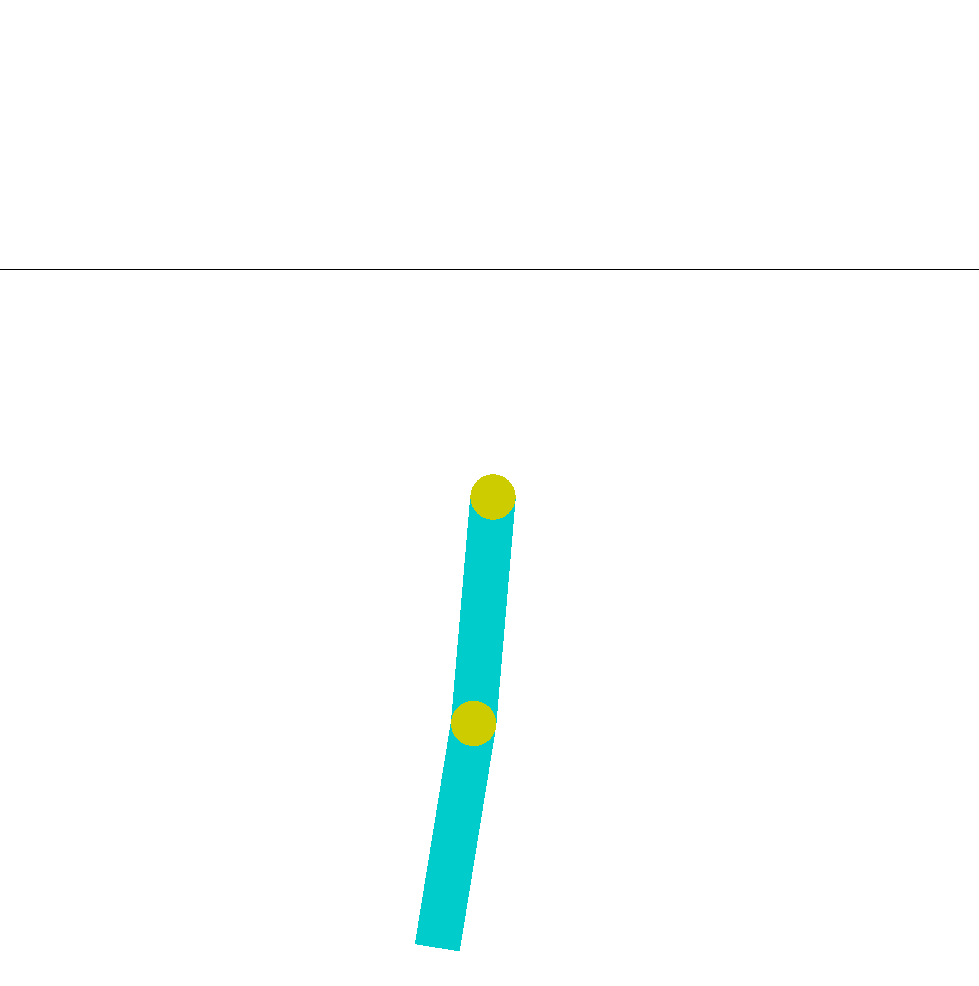
\includegraphics[width=0.9\linewidth]{img11}
    \caption{initial status}
  \end{subfigure}%
    \begin{subfigure}{0.33\textwidth}
    \centering
    
\includegraphics[width=0.9\linewidth]{img12}
    \caption{middle status}
  \end{subfigure}%
    \begin{subfigure}{0.33\textwidth}
    \centering
    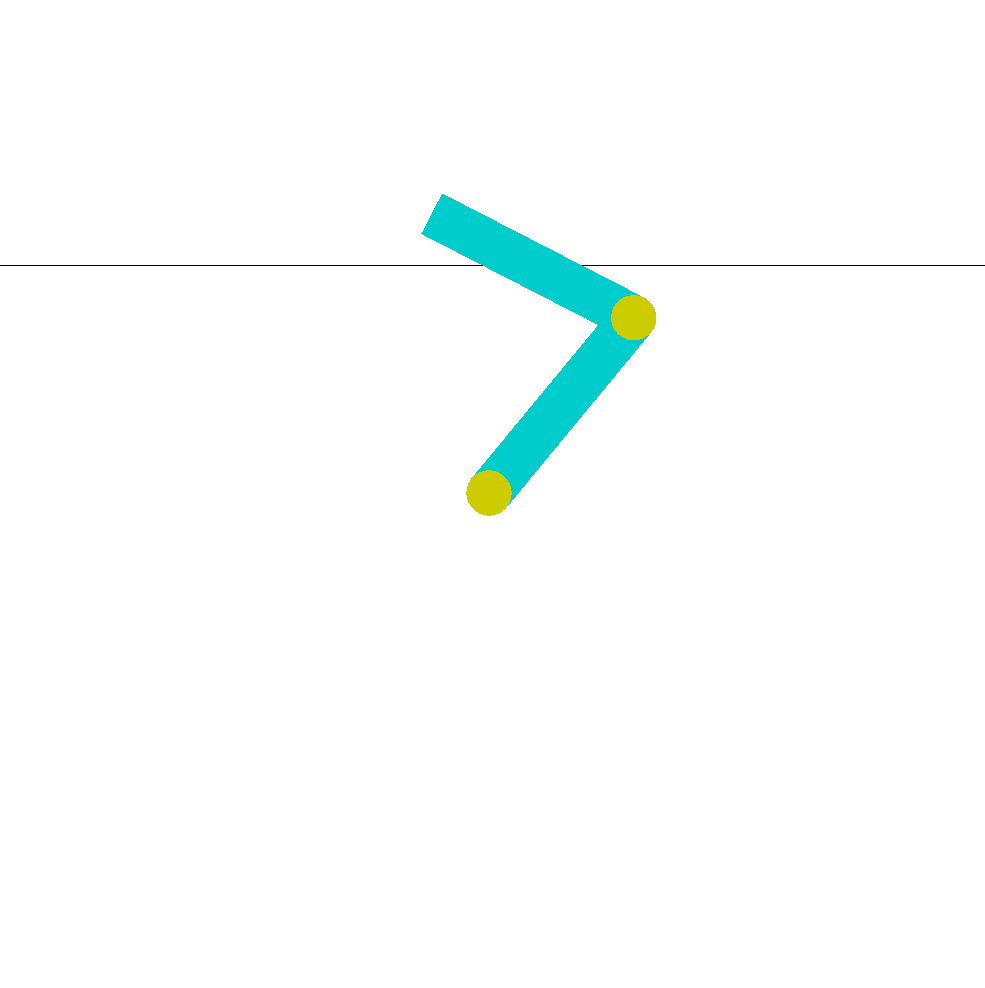
\includegraphics[width=0.9\linewidth]{img13}
    \caption{successful status}
  \end{subfigure}%
  \caption{Three status of Acrobot}
\end{figure}



%%%%%%%%%%%%%%%%%%%%%%
\section{Algorithm}

In this part, I will introduce the details about using Double Deep Q-Network to approximate the Q function. I design the double DQN algorithm following the algorithm in the deep Q-network paper \citep{mnih2015human}, where two neural networks (current-net \& target-net) are introduced to approximate and update function $Q$. According to \citet{van2016deep}, the only difference between DQN and double DQN is that in DQN, we compute the target $Y_t^{DQN}$:
$$
Y_t^{DQN} = R_{t+1} + \gamma max_a Q_{\mathrm{target}}(S_{t+1}, a);
$$
while in double DQN, we compute the target $Y_t^{\mathrm{DoubleQ}}$:
$$
Y_t^{\mathrm{DoubleQ}} = R_{t+1} + \gamma Q(S_{t+1}, \mathrm{argmax}_a Q_{\mathrm{target}}(S_{t+1}, a));
$$
The algorithm in \citep{mnih2015human} also use experience replay (i.e. remember M states and update the neural network only using data in a size-$m$ batch, where $m \ll M$ ) to avoid overfitting and make the algorithm more robust. Besides, I made several adjustments to the original algorithm: 
(a). In order to accelerate the algorithm, we only update the current-net every 100 iterations;
(b). We use soft-update to reset the target-net to further reduce the possibility of overfitting;
(c). We stop training before going through all episodes if the model perform good enough.
All the details of the double DQN algorithm can be found in Algorithm 1.

\begin{algorithm}[H]
\caption{Pseudo Code for Double DQN}
\begin{algorithmic} [1]
\STATE Initialize replay memory D to capacity 10000, batch size = 50; 
\STATE Create two NN (current-net \& target-net) as the initial function approximation of $Q(s, a)$ and $Q_{\mathrm{target}}(s, a)$.
\FOR{Episode $= 1, \cdots , 2000$}
    \STATE Initialize state $S$;
    \STATE Set $\mathrm{TotalStep} = 0$;
    \FOR{t $= 1, \cdots , 2000$}
    \STATE Choose action A based on $\epsilon$-greedy algorithm with $\epsilon$;
    \STATE Execute $A$ in environment, observe $R$, $S^{'}$, and $\mathrm{terminated}$ (i.e. termination status);
    \STATE Store and fresh the memory with $[S, A, R, S^{'}, \mathrm{terminated}]$;
    \STATE $\mathrm{TotalStep} = \mathrm{TotalStep}+1$;
    
    ******************* update current-net *********************
    \IF{$\mathrm{TotalStep}\ \% \ 100 == 0$}
    \STATE Randomly select a batch of state-action pairs from memory;
    \FOR{$[S, A, R, S^{'}, \mathrm{Done}]$ in batch}
      \STATE Compute $A_{\max} = \mathrm{argmax}_a Q(S^{'}, a)$;
      \STATE Compute $\hat{Q}_{\mathrm{target}}(S, A) = R + \gamma Q_{\mathrm{target}}(S^{'}, A_{\max})$;
      \STATE Train current-net by minimizing the square error between $Q_{\mathrm{target}}(S,A)$ and $\hat{Q}_{\mathrm{target}}(S,A)$;
    \ENDFOR
    \ENDIF
    
    ****************** soft-update target-net *******************
    \IF{$\mathrm{TotalStep}\ \% \ 2000 == 0$}
    \STATE Get NN parameters $\Theta_{\mathrm{current}}$ and $\Theta_{\mathrm{target}}$;
    \STATE $\Theta_{\mathrm{target}} \leftarrow \tau \Theta_{\mathrm{current}} + (1 - \tau) \Theta_{\mathrm{target}}$;
    \ENDIF
    \STATE Update state $S = S^{'}$
    \STATE Break if the episode is terminated.
    \ENDFOR
    \STATE Break if the averaged rewards of the past few episodes is good enough.
\ENDFOR


\end{algorithmic}
\end{algorithm}



By experiments, I eventually choose $\epsilon = 0.1$, $\gamma = 0.9$, $\tau = 0.5$. We model the current-net and target net using:  \\
(1). Single layer neural network with input size 6, output size 3, and linear function as the activation function.  \\
(2). Two layers neural network with input size 6, hidden layer size 10, output size 3, RELU and linear functions as the two activation functions. 

Finally, mean squared error is used as evaluation criteria and learning rate is chosen to be 0.001 under `Adam' optimizer. Keras is used to build the double DQN under Python.



%%%%%%%%%%%%%%%%%%%%%%
\section{Results}

\subsection{Training Results}

We compare the results between the two neural network structures in this section. From Figure 2, we find that the 2-layer model is not as stable as the single-layer model since it has larger variance of reward than the single-layer model. Meanwhile, the training procedure of the 2-layer model stops after 800 episodes, while the single-layer model only need around 300 episodes in order to perform well. A more detailed training summary can be found in Table 1.


\begin{table}[h]
\begin{center}
\vspace{1mm}
\begin{tabular}{ccccc}
\hline
 \hline
structure & total episodes &  comp. time [min]  & avg. rewards & avg. rewards (last 100 episodes)   \\
 \hline 
single-layer & 328 & 6.1 & -635.64 & -122.58 \\
2-layer & 846 & 14.53 & -554.56 & -241.30 \\
 \hline
 \hline
\end{tabular}
\end{center}
\vspace{-1em}
\caption{Summary of training for the two models}
\end{table}




\begin{figure}[h]
  \begin{subfigure}{0.5\textwidth}
    \centering
    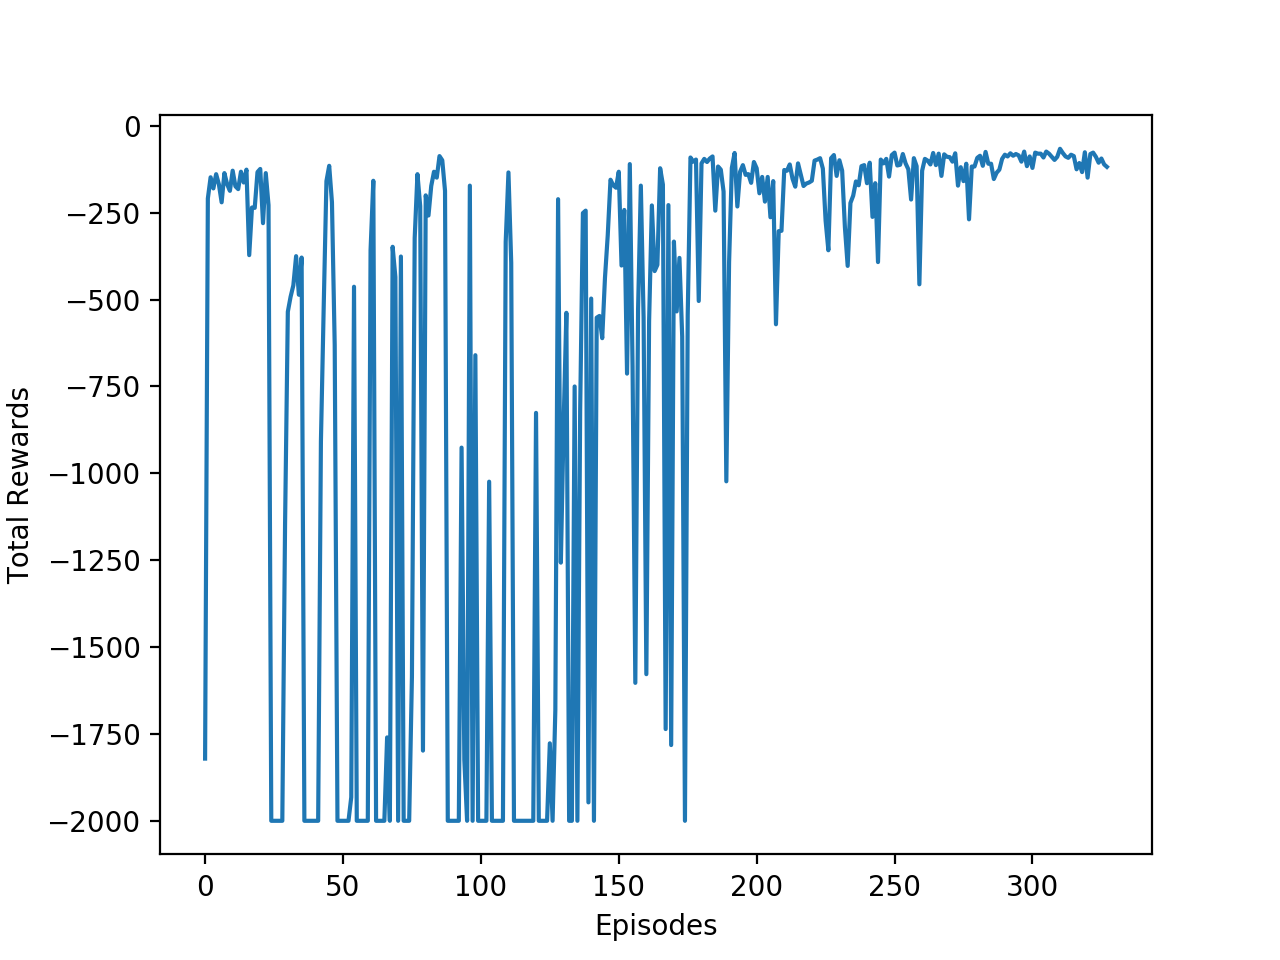
\includegraphics[width=1.0\linewidth]{train_reward_1layer_1.png}
    \caption{NN with single layer}
  \end{subfigure}%
    \begin{subfigure}{0.5\textwidth}
    \centering
    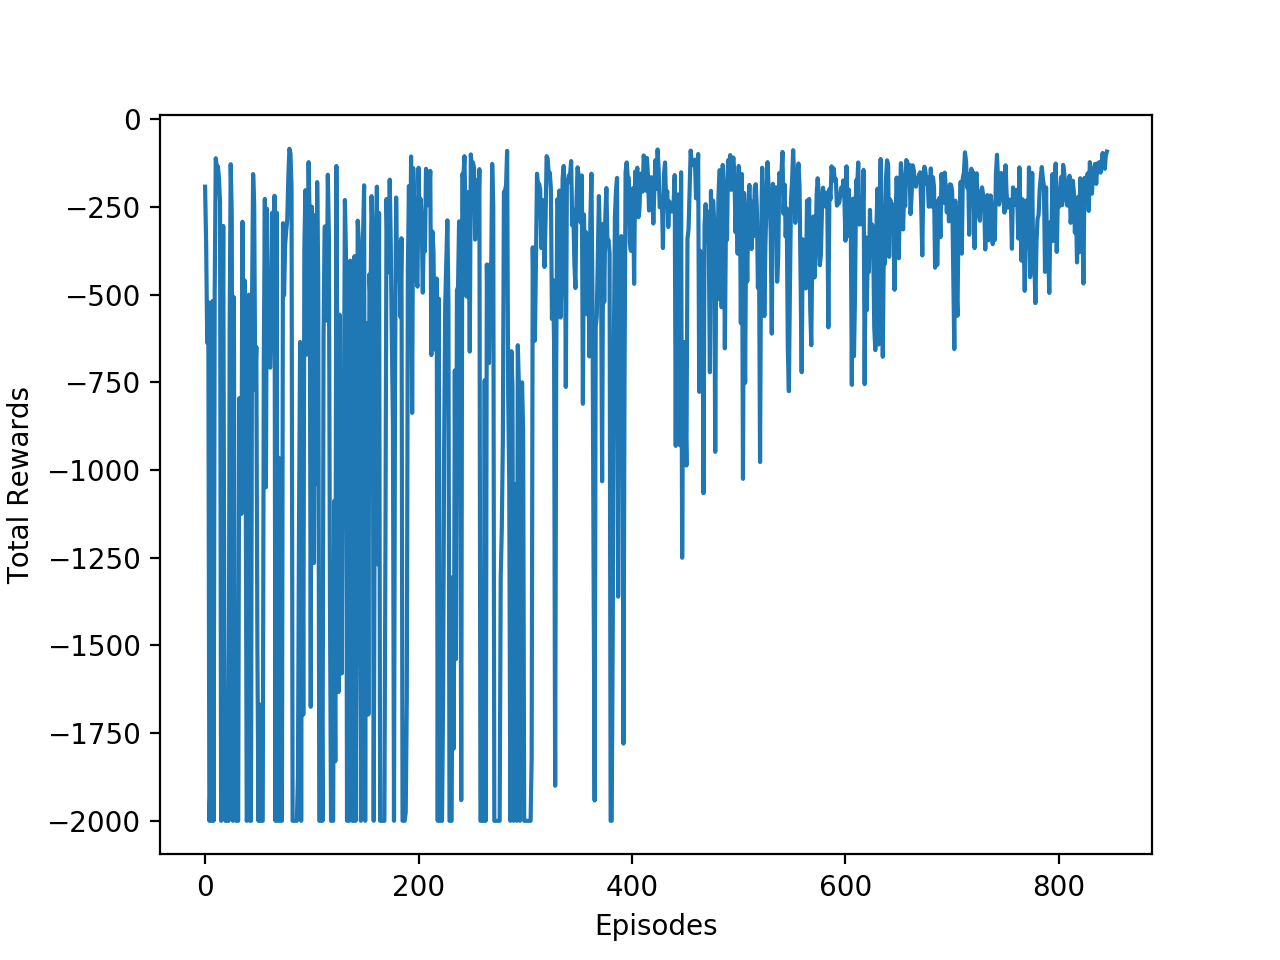
\includegraphics[width=1.0\linewidth]{train_reward_2layers_1.png}
    \caption{NN with two layers}
  \end{subfigure}%
  \caption{Total rewards (training) for different network structure}
\end{figure}




\subsection{Testing Results}

The histogram of testing results for the two trained models for 500 testing episodes can be found in Figure 3. It's easy to see that both models perform pretty well in terms of the total rewards. We can also see from Table 2 that, single-layer model is relatively better than the 2-layer model in terms of both mean and variance. Also, the single-layer model achieve the goal in 500 steps for every episodes, which is really impressive.


\begin{table}[h]
\begin{center}
\vspace{1mm}
\begin{tabular}{ccccc}
\hline
 \hline
structure & mean &  median   & std. dev. & failed ratio (in 500 steps)  \\
 \hline 
single-layer & -99.4 & -93.0 & 30.9 & $0.0\%$  \\
2-layer & -115.0 & -105.0 & 73.9 & $0.4\%$  \\
 \hline
 \hline
\end{tabular}
\end{center}
\vspace{-1em}
\caption{Summary of testing for the two models}
\end{table}




\begin{figure}[h]
  \begin{subfigure}{0.5\textwidth}
    \centering
    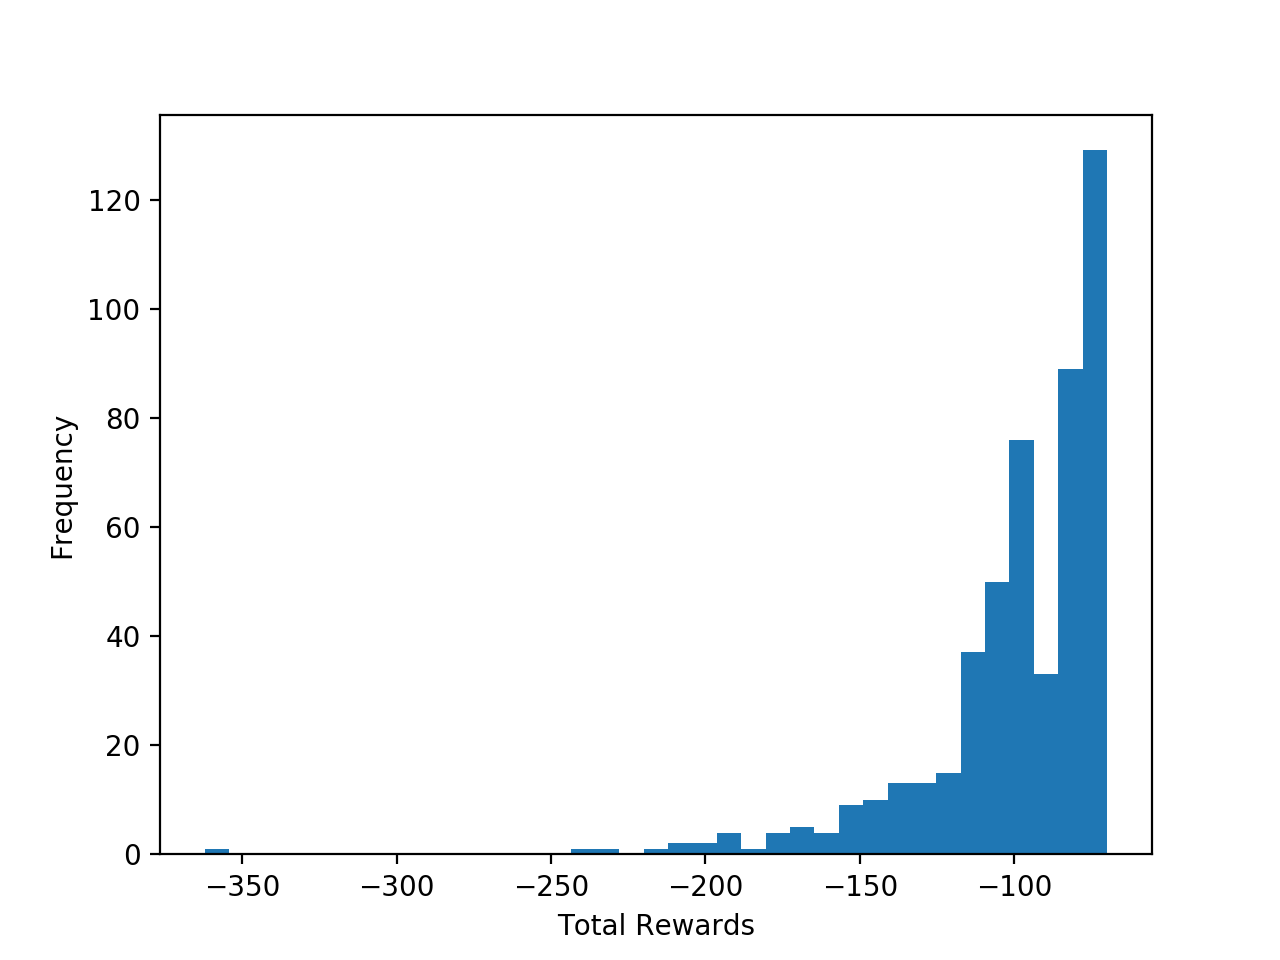
\includegraphics[width=1.0\linewidth]{histogram_m1.png}
    \caption{NN with single layer}
  \end{subfigure}%
    \begin{subfigure}{0.5\textwidth}
    \centering
    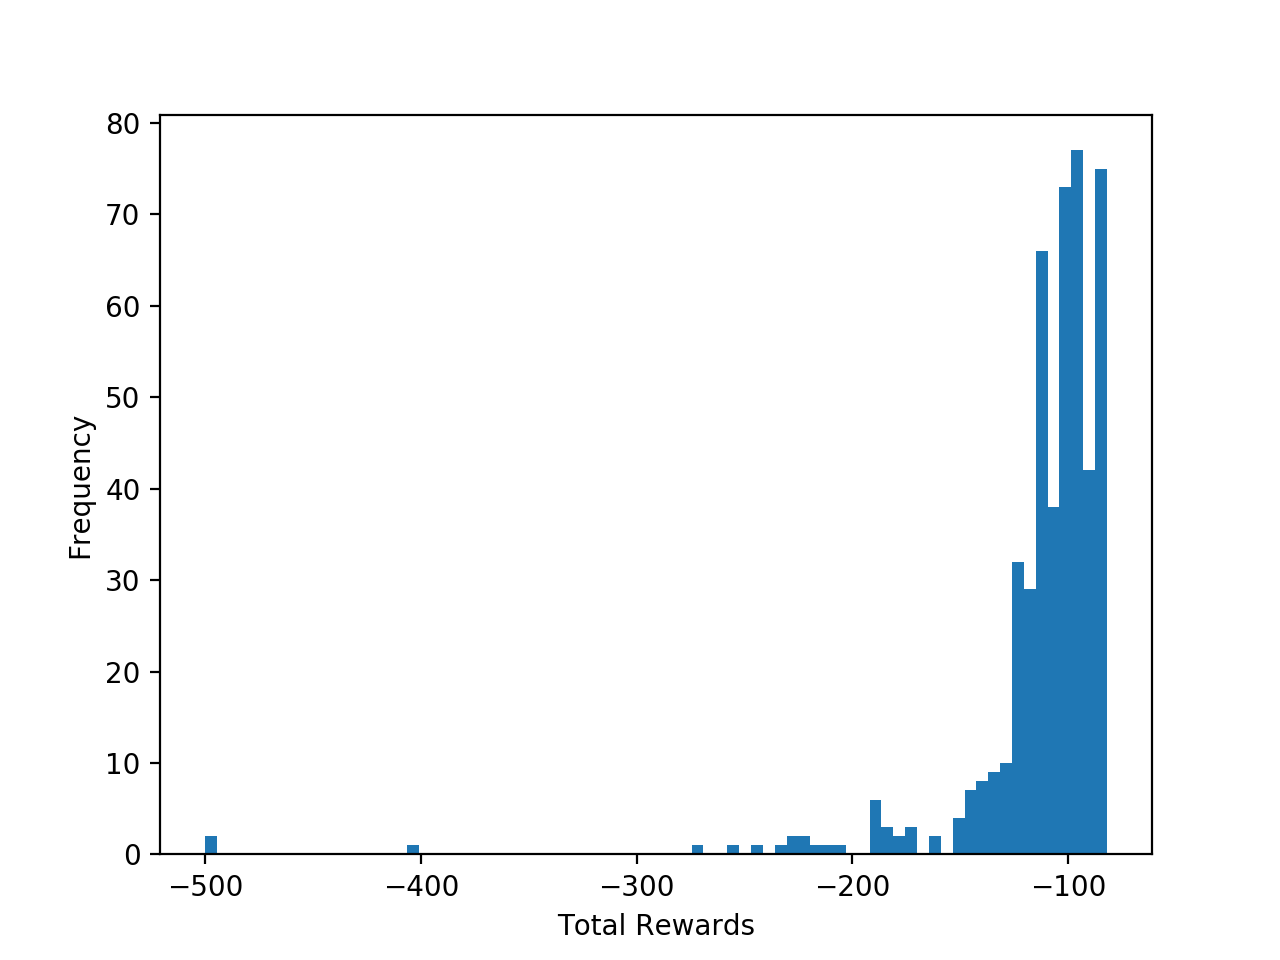
\includegraphics[width=1.0\linewidth]{histogram_m2.png}
    \caption{NN with two layers}
  \end{subfigure}%
  \caption{Histogram of the total rewards (500 testing episodes) for different network structure}
\end{figure}




%%%%%%%%%%%%%%%%%%%%%%
\section{Further Improvements}

The results that I presented in this report is the best attempts. In fact, I faced several problems when I train the models:
\begin{itemize}
\item The parameter settings is really difficult to tune and the models are easily overfitted. 
\item Using more complex neural networks (more than 2 layers) is more likely to overfit in the end, the testing results for a 3-layer neural networks is really unstable.
\item It is likely that the performance of the model becomes better at first and then get worse when there are too many episodes, that why I need to use the early stop trick.
\end{itemize}
The possible improvements are:
\begin{itemize}
\item Make more efforts on tuning the hyper-parameters since the parameter setting is important for the training.
\item Compare the double DQN algorithms with other deep reinforcement learning algorithms (e.g. DQN, Actor-Critic, etc.).
\item Use more reasonable reward function (I notice that the reward function is ?1 for all states and actions).
\end{itemize}





%%%%%%%%%%%%%%%%%
\bibliographystyle{apalike}
%\nocite{*}
\bibliography{ref}


\end{document}













